\documentclass[12pt]{article}
\usepackage{graphicx, float}
\usepackage[utf8]{inputenc}
\usepackage[T2A]{fontenc}
\usepackage[serbianc]{babel}
\usepackage {amsmath, amssymb, amsthm}
\graphicspath{{figures/}}
\usepackage[shortlabels]{enumitem}
\usepackage{hyperref}
\hypersetup{colorlinks=true, linkcolor=black, urlcolor=blue, breaklinks=true}
\usepackage{xurl}

%   formatting
\usepackage[a4paper, top=1cm, bottom=1.5cm, left=2cm, right=1cm, heightrounded]{geometry}
\renewcommand{\baselinestretch}{1.15}
\setlength{\parindent}{0pt}
\setlength{\parskip}{0.8em}

\title{Дипломски Рад}
\author{Лазар Попадић}
\date{Август 2024}
%\maketitle

\begin{document}
\tableofcontents
\newpage

\section{Теорија}

\subsection{Паралелни манипулатори}
Роботски манипулатори су уређаји који врше манипулацију објеката у простору. Главна функција манипулатора подразумева задатке који захтевају брзо и прецизно позиционирање предмета рада. Манипулатори су мехатроничарски уређаји који се састоје из механичког подсистема, управљачке и енергетске електронике. Према типу механичког подсистема, манипулатори се деле на: серијске, паралелне и мобилне.

Кинематски ланац представља низ крутих сегмената који су повезани преко зглобова. Прости кинематски ланци су они код којих ниједан сегмент није повезан са више од 2 сегмента. Механички подсистем серијских манипулатора представља прости кинематски ланац код којих су сегменти базе и крајњег ефектора повезани са 1, а сви остали са 2 сегмента [1].

\begin{figure}[H]
    \centering
    \includegraphics[width=12cm]{figures/abb_irb_140.jpg}
    \caption{Серијски манипулатор антропоморфне конфигурације \textit{ABB IRB} 140 [2]}
    \label{fig:серијски_манипулатор}
\end{figure}

Затворени кинематски ланац се добија када је један од сегмената, али не и база, повезан са 3 или више сегмента [1]. Механички подсистем паралелних манипулатора представља затворени кинематски ланац, код којег је крајњи ефектор повезан са базом преко више од једног кинематског ланца. Свака веза базе и крајњег ефектора садржи барем један актуатор.

\begin{figure}[H]
    \centering
    \includegraphics[width=12cm]{figures/abb_irb_360.jpg}
    \caption{Паралелни манипулатор делта конфигурације \textit{ABB IRB} 360 [2]}
    \label{fig:паралелни_манипулатор}
\end{figure}

За разлику од серијских, сви актуатори паралелних манипулатора могу бити на непокретном сегменту, односно бази. То омогућава да, без негативних последица на крутост ланца, сегменти буду лакши него код серијских манипулатора. Додатна предност је то што се оптерећење које делује на крајњи ефектор разлаже на сваки ланац којим је повезан са базом. Из тога закључујемо да су главне предности паралелних манипулатора у односу на серијске::
\begin{itemize}
    \item већа крутост кинематског ланца
    \item мања маса манипулатора
    \item већа носивост
    \item боља прецизност, као последица мањих деформација
\end{itemize}
С обзиром да је код паралелних манипулатора крајњи ефектор повезан са базом преко више од 1 кинематског ланца, кинематска анализа је знатно сложенија. Такође, сваки кинематски ланац уноси и одређена кинематска ограничења, због којих је радни простор мањи него код серијских манипулатора. 
Главне мане паралелних манипулатора су:
\begin{itemize}
    \item мањи радни простор
    \item сложенија кинематска и динамичка анализа
\end{itemize}

\subsubsection{Сингуларне конфигурације}
Сингуларне конфигурације су одређени положаји крајњег ефектора, за које паралелни роботи губе своју инхерентну бесконачну крутост, и у којима крајњи ефектор има неконтролисане степене слободе [1]. Типови кинематских сингуларитета:
\begin{itemize}
    \item Тип 1. За ненулти вектор улазних брзина, крајњи ефектор се не креће.
    \item Тип 2. Крајњи ефектор се креће при нултом вектору улазних брзина.
    \item Тип 3. Комбинација сингуларитета типа 1 и 2. Могуће је кретање крајњег ефектора без кретања улазних сегмената, и обрнуто, могуће је кретање улазних сегмената без кретања крајњег ефектора.
\end{itemize}

\subsubsection{Кинематска анализа}
Кинематска анализа манипулатора обухвата проучавање кретања свих сегмената. Од кључног значаја су односи између координата, брзина и убрзања улазних чланова и крајњег ефектора. Кинематски проблем се дели на директни и индиректни.

Директни кинематски проблем обухвата проналажење кинематских параметара крајњег ефектора за задате улазне параметре. Решење за паралелне манипулаторе зависи од конфигурације, односно, не мора бити јединствено. Аналитичка метода за решавање проблема директне кинематике представља решавање система векторских једначина. Почевши од система за положај, формулишу се векторске једначине које изражавају вектор положаја врха крајњег ефектора преко карактеристичних вектора. Карактеристични вектори описују положај једног сегмента кинематског ланца. Карактеристични вектор је постављен у правцу сегмента, а његов интензитет представља дужину тог сегмента.

Након решавања система за положај, векторске једначине се диференцирају по времену како би се добио систем за брзину. Након тога се опет диференцирају како би се добио систем за убрзање.

\begin{figure}[H]
    \centering
    \includegraphics[width=8cm]{figures/4bar.png}
    \caption{Пример директног кинематског проблема}
    \label{fig:дир_кин_пример}
\end{figure}

Инверзни кинематски проблем обухвата проналажење параметара улазних сегмената за жељени положај крајњег ефектора. Као и код директне, решење не мора бити јединствено. Иста метода за решавање директне кинематике се може применити и за инверзну кинематику.

\subsubsection{Динамичка анализа}
Динамичка анализа представља одређивање односа између кинематских параметара и оптерећења које делују на манипулатор. Динамика обухвата постављање једначина кретања, које описују како се манипулатор креће под утицајем оптерећења. Оптерећења могу бити спољашња и унутрашња. Спољашња настају услед утицаја спољашњих сила и момената, на пример гравитациона сила предмета рада и силе улазних актуатора. Унутрашња оптерећења обухватају реакције веза у зглобовима кинематског ланца.

Једначине кретања могу бити исписане помоћу Њутнових закона кретања. Оне су допуњене Даламберовим принципом који уводи инерцијалну силу: $\vec{F}_{in} - m\vec{a} = 0,$ и момент силе: $\vec{M}_{in} - I\vec{\alpha} = 0$. Даламберов принцип нам омогућава да динамичке проблеме посматрамо као статичке.

Динамичка анализа обухвата директан и инверзни динамички проблем. Директан проблем обухвата израчунавање трајекторије, брзине и убрзања крајњег ефектора на основу задатих улазних оптерећења. Инверзан проблем обухвата израчунавање потребних улазних оптерећења на основу задате трајекторије, брзине и убрзања крајњег ефектора.

Решавање проблема динамике обухвата вршење декомпозиције кинематског ланца, односно формирање \textit{Free-Body Diagram}-а. Затим се формирају једначине кретања за ротационо и транслаторно кретање сваког сегмента. При чему сила реакције везе којом један сегмент делује на други је истог интензитета и правца, а супротног смера у односу на силу којом тај други сегмент делује на први, на пример: $\vec{F_{12}} = -\vec{F_{21}}$. Формирањем тих једначина добија се систем, чије решење представља решење динамичког проблема.

\begin{figure}[H]
    \centering
    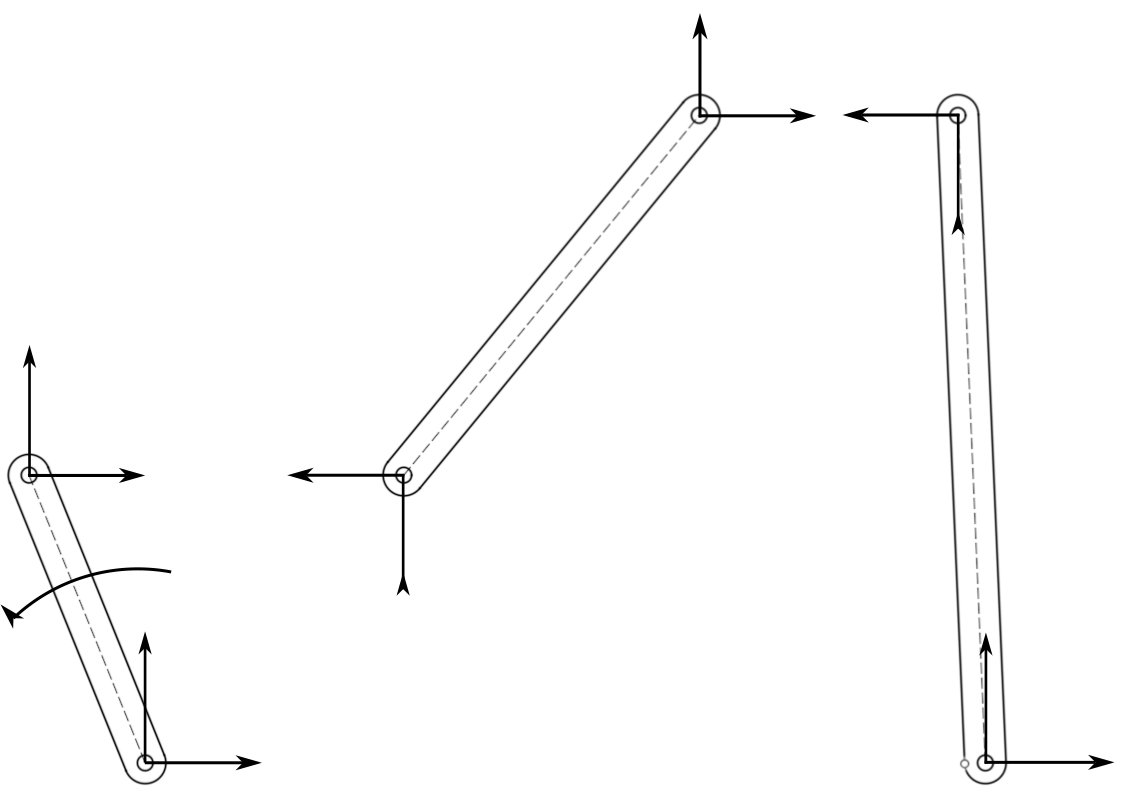
\includegraphics[width=14cm]{figures/4bar_fbd.png}
    \caption{Пример \textit{Free-Body Diagram}-а}
    \label{fig:фбд_пример}
\end{figure}

\subsection{Машине једносмерне струје}
Машине једносмерне струје, у наставку МЈС, су електромеханички претварачи, који улазну електричну енергију претварају у механички рад. Састоје се из статора и ротора(арматуре). Статор успоставља побудно магнетно поље, због чега се назива и побуда. Кроз ротор се, преко четкица и комутатора, пропушта улазна арматурна струја. По принципу Лоренцовог закона $\vec F=Q(\vec v \times \vec B)$, индукује се сила која делује на ротор. Комутатор врши промену смера арматурне струје у зависности од положаја ротора, и тиме омогућава да Лоренцова сила увек делује у истом смеру, односно обезбеђује константан обртни момент мотора. Због Фарадејевог закона и Ленцовог правила $e_a=-N\dfrac{\partial\phi }{\partial t}$, обртање ротора индукује електромоторну силу супротног смера.

\begin{figure}[H]
    \centering
    \includegraphics[width=12cm]{figures/ekv_kolo_armatura.png}
    \caption{Еквивалентно коло арматуре МЈС}
    \label{fig:коло_арматуре}
\end{figure}


\subsubsection{Динамички модел МЈС}
Модел МЈС се састоји из 2 подсистема: механичког и електричног, који међусобно интерагују. Посматраћемо МЈС која има сталну побуду јачинe магнетног флукса $\psi _f$. Модел се састоји из 3 диференцијалне једначине: напонске равнотеже арматурног навоја, механичке равнотеже и релације механичке брзине обртања и угла ротора [5]. Као и из 2 алгебарске једначине: дефиниције електромагнетног момента и дефиниције индуковане електромоторне силе.
\begin{equation}
    u_a-e_a=R_ai_a+L_a\dfrac{di_a}{dt}
\end{equation}
\begin{equation}
    m_e-m_m=J_m \dot\omega+B_m\omega
\end{equation}
\begin{equation}
    \dfrac{d\theta}{dt}=\omega
\end{equation}
\begin{equation}
    m_e=\psi _fi_a
\end{equation}
\begin{equation}
    e_a=\psi _f\omega
\end{equation}
\newpage
Значења величина математичког модела МЈС:
\begin{itemize}
    \item $u_a$ - улазни арматурни напон
    \item $e_a$ - индукована електромоторна сила
    \item $R_a$ - електрична отпорност арматурног намотаја
    \item $i_a$ - арматурна струја
    \item $L_a$ - индуктивност арматурног намотаја
    \item $m_e$ - електромагнетни моменат
    \item $m_m$ - моменат оптерећења погона
    \item $J_m$ - моменат инерције обртних маса
    \item $\omega$ - угаона брзина арматуре
    \item $B_m$ - коефицијент пригушења брзине услед трења
    \item $\theta$ - угао ротора
    \item $\psi _f$ - јачина магнетног флукса побуде
\end{itemize}

\subsubsection{МЈС у стационарном стању}
Стационарно стање МЈС подразумева режим рада у којем су изводи променљивих стања по времену једнаки нули. Односно, арматурни напон и струја, моменат оптерећења и угаона брзина су константни. Овакво стање система је равнотежно и омогућава нам да лакше увидимо законитости утицаја улазних величина на излазне. Из једначина (2) и (4) следи:
\begin{equation}
    i_a=\dfrac{B_m\omega+m_m}{\psi _f}
\end{equation}
Уврштавањем (5) и (6) у (1):
\begin{equation}
    \omega(1+\dfrac{R_aB_m}{\psi _f^2})=\dfrac{u_a}{\psi _f}-\dfrac{R_am_m}{\psi _f^2}
\end{equation}
<<<<<<< HEAD
Коефицијент пригушења брзине $B_m$ је типично занемарљив [3], због чега уводимо апроксимацију $B_m=0$. Тиме (6) и (7) постају:
=======
С обзиром да је коефицијент пригушења брзине $B_m$ типичног реда величине $10^{-6}$, можемо увести апроксимацију $B_m=0$. Тиме (6) и (7) постају:
>>>>>>> 72bc6d8a9125a83ded69a8fc6b1fd5fd3258f344
\begin{equation}
    i_a=\dfrac{m_m}{\psi _f}
\end{equation}
\begin{equation}
    \omega=\dfrac{u_a}{\psi _f}-\dfrac{R_am_m}{\psi _f^2}
\end{equation}
<<<<<<< HEAD
Из (9) се може закључити да повећањем арматурног напона, угаона брзина линеарно расте, а повећањем момента оптерећења угаона брзина линеарно опада. Из тог закључка следи и идеја о регулацији брзине МЈС променом улазног арматурног напона [6].
=======
Из (9) се може закључити да повећањем арматурног напона, угаона брзина линеарно расте, а повећањем момента оптерећења угаона брзина линеарно опада. Из тог закључка следи и идеја о регулацији брзине МЈС променом улазног арматурног напона.
>>>>>>> 72bc6d8a9125a83ded69a8fc6b1fd5fd3258f344

\begin{figure}[H]
    \centering
    \includegraphics[width=15cm]{figures/k-ka_bdc.drawio.png}
    \caption{Механичка карактеристика МЈС}
    \label{fig:карактеристика_мјс}
\end{figure}

\subsection{PID регулација}
Регулација процеса представља управљање променљивама од значаја на основу управљачког алгоритма. Управљачки алгоритам представља функцију на основу које се генерише управљачки сигнал, на основу улазних сигнала. Основни захтеви регулације су: стабилност, тачност и брзина одзива. Два основна типа регулације су у затвореној и отвореној петљи. Односно, управљање са повратном спрегом и без повратне спреге. 

Регулација у отвореној петљи (open-loop control, non-feedback control loop) представља управљање у којем вредности излазних сигнала и сметњи немају утицај на управљачке сигнале. Овакви системи немају могућност отклањања грешака које су настале услед спољашњих поремећаја који делују на систем, или услед неидеалног познавања функционисања система. Системи који користе регулацију у отвореној петљи су спори системи који не захтевају велику прецизност и поновљивост.

\begin{figure}[H]
    \centering
    \includegraphics[width=14cm]{figures/open_loop.drawio.png}
    \caption{Блок шема управљања у отвореној спрези}
    \label{fig:отворена_спрега}
\end{figure}

Регулација у затвореној петљи (closed-loop control, feedback control loop) представља управљање у којем вредност управљачких сигнала зависи од разлике референтне(жељене) вредности и стварне вредности излазног сигнала. Овакви системи не захтевају идеално познавање управљаног система и имају могућност отклањања грешака услед спољашњих поремећаја.

\begin{figure}[H]
    \centering
    \includegraphics[width=15cm]{figures/closed_loop.drawio.png}
    \caption{Блок шема управљања у затвореној спрези}
    \label{fig:затворена_спрега}
\end{figure}

\subsubsection{Пропорцијално дејство}
<<<<<<< HEAD
Регулација на основу пропорцијалног дејства, односно P регулатори, представљају најједноставнији тип регулације са затвореном повратном спрегом. Управљачки сигнал представља сигнал грешке помножен фактором појачања пропорцијалног дејства [4]:
=======
Регулација на основу пропорцијалног дејства, односно P регулатори, представљају најједноставнији тип регулације са затвореном повратном спрегом. Управљачки сигнал представља сигнал грешке помножен фактором појачања пропорцијалног дејства:
>>>>>>> 72bc6d8a9125a83ded69a8fc6b1fd5fd3258f344
\begin{equation}
    u_{(t)} = K_p e_{(t)},
\end{equation}
где $K_p$ предстаља фактор појачања пропорцијалног дејства, $u_{(t)}$ је управљачки сигнал, а $e_{(t)}$ је сигнал грешке. Сигнал грешке је једнак разлици референтне вредности и измерене вредности излаза, односно:
\begin{equation}
    e_{(t)}=y_{ref(t)} - y_{mer(t)}
\end{equation}
Функција преноса P регулатора у комплексном фреквенцијском домену је:
\begin{equation}
    G_{p(s)} = \dfrac{U_{(s)}}{E_{(s)}} = K_p
\end{equation}
\begin{figure}[H]
    \centering
    \includegraphics[width=13cm]{figures/p.drawio.png}
    \caption{Одзив P регулатора на одскочни сигнал грешке}
    \label{fig:P_одзив}
\end{figure}

\subsubsection{Интегрално дејство}
<<<<<<< HEAD
Регулација на основу интегралног дејства, односно I регулатори, су настали како би отклонили главну ману P регулатора. Та мана је могућност потпуног отклањања грешке у стационарном стању. I дејство негативно утиче на брзину одзива и на стабилност система. Управљачки сигнал I регулатора представља одређен интеграл сигнала грешке по времену, помножен фактором појачања интегралног дејства $K_i$ [4]:
=======
Регулација на основу интегралног дејства, односно I регулатори, су настали како би отклонили главну ману P регулатора. Та мана је могућност потпуног отклањања грешке у стационарном стању. I дејство негативно утиче на брзину одзива и на стабилност система. Управљачки сигнал I регулатора представља одређен интеграл сигнала грешке по времену, помножен фактором појачања интегралног дејства $K_i$:
>>>>>>> 72bc6d8a9125a83ded69a8fc6b1fd5fd3258f344
\begin{equation}
    u_{(t)} = K_i\int_{0}^{t}e_{(t)}dt
\end{equation}
Функција преноса I регулатора у комплексном фреквенцијском домену је:
\begin{equation}
    G_{i(s)} = \dfrac{U_{(s)}}{E_{(s)}} = \dfrac{K_i}{s}
\end{equation}
\begin{figure}[H]
    \centering
    \includegraphics[width=13cm]{figures/i.drawio.png}
    \caption{Одзив I регулатора на одскочни сигнал грешке}
    \label{fig:I_одзив}
\end{figure}

\subsubsection{Диференцијално дејство}
<<<<<<< HEAD
Регулација на основу диференцијалног дејства, односно D регулатори, су настали како би отклонили мане I регулатора. Односно, како би убрзали одзив у прелазном режиму и смањили осцилације у устаљеном стању. Управљачки сигнал D регулатора представља извод сигнала грешке по времену, помножен фактором појачања диференцијалног дејства $K_d$ [4]:
=======
Регулација на основу диференцијалног дејства, односно D регулатори, су настали како би отклонили мане I регулатора. Односно, како би убрзали одзив у прелазном режиму и смањили осцилације у устаљеном стању. Управљачки сигнал D регулатора представља извод сигнала грешке по времену, помножен фактором појачања диференцијалног дејства $K_d$:
>>>>>>> 72bc6d8a9125a83ded69a8fc6b1fd5fd3258f344
\begin{equation}
    u_{(t)} = K_d\dfrac{de_{(t)}}{dt}
\end{equation}
Функција преноса D регулатора у комплексном фреквенцијском домену је:
\begin{equation}
    G_{d(s)} = \dfrac{U_{(s)}}{E_{(s)}} = K_ds
\end{equation}
\begin{figure}[H]
    \centering
    \includegraphics[width=13cm]{figures/d.drawio.png}
    \caption{Одзив D регулатора на сигнал грешке типа рампа}
    \label{fig:D_одзив}
\end{figure}

\subsubsection{PID}
PID регулатор настаје комбиновањем сва три претходно наведена дејства. Подешавањем фактора појачања пропорцијалног, диференцијалног и интегралног дејства могу се обезбедити жељене перформансе система.
Управљачки сигнал PID регулатора је:
\begin{equation}
    u_{(t)} = K_p e_{(t)} + K_i\int_{0}^{t}e_{(t)}dt + K_d\dfrac{de_{(t)}}{dt}
\end{equation}
Функција преноса PID регулатора у комплексном фреквенцијском домену је:
\begin{equation}
    G_{pid(s)} = \dfrac{U_{(s)}}{E_{(s)}} = K_p + \dfrac{K_i}{s} + K_ds
\end{equation}

\begin{figure}[H]
    \centering
    \includegraphics[width=18cm]{figures/pid.drawio.png}
    \caption{Блок шема PID регулатора у затвореној спрези}
    \label{fig:PID_затворена_спрега}
\end{figure}

<<<<<<< HEAD
\subsection{PSO алгоритам}
PSO (\textit{Particle swarm optimization}) је... TODO: наставак
\begin{itemize}
    \item о оптимизацији, минимизација функције у зависности од параметара
    \item природни алгоритми, њихове предности и мане
    \item све о параметрима псо: позиција, брзина, когнитивни, социјални, инерција(+побољшање)
\end{itemize}

\newpage
\section{Литература}
\begin{enumerate}[start=1,label={[\arabic*]}]
\item Parallel Robots (Second Edition), Jean-Pierre Merlet, Springer 2006
\item \url{https://new.abb.com/en}
\item \url{https://support.maxongroup.com/hc/en-us/articles/360013761160-Motor-data-and-simulation}
\item \url{http://www.automatika.ftn.uns.ac.rs/images/predmeti/Sistemi%20automatskog%20upravljanja%20-%20mehatronika/Predavanja/10_Regulacija.pdf}, Системи аутоматског управљања,
др Александар Ристић, редовни професор, др Владимир Бугарски, доцент
\item \url{https://www.keep.ftn.uns.ac.rs/regulisani-elektromotorni-pogoni/specifikacija/specifikacija-predmeta/}, Регулисани електромоторни погони, др Дарко Марчетић, редовни професор, МСц Владимир Поповић, доцент
\item Збирка задатака из електричних машина за студијски програм мехатроника, др Дејан Јеркан, Барбара Вујков, Нови Сад, ФТН 2020
\end{enumerate}

=======
>>>>>>> 72bc6d8a9125a83ded69a8fc6b1fd5fd3258f344
\end{document}
